\graphicspath{{2babylon/pics/}}

\section{Babylon/Mesopotamia}

\begin{minipage}[t]{0.53\linewidth}\vspace{0pt}
	\emph{Babylon} was an ancient city located near modern-day Baghdad, Iraq. The term also serves as a shorthand for the many Mesopotamian\footnotemark{} empires/civilizations dating back at least to 3000\BC{}: Sumeria, Akkadia, Babylonia, etc.
	\smallbreak
	Babylonians used \emph{cuneiform} (wedge-shaped) script, typically indentations on clay tablets. Most recovered tablets date from the time of Hammurabi (c.\,1800\BC) or the Seleucid dynasty (c.\,300\BC) which ruled after the conquests of Alexander the Great.
	\smallbreak
	Mathematical tablets are of two main types: tables of values (multiplication, reciprocals, measures) and worked problems.
\end{minipage}
\hfill
\begin{minipage}[t]{0.46\linewidth}\vspace{0pt}
	\flushright
	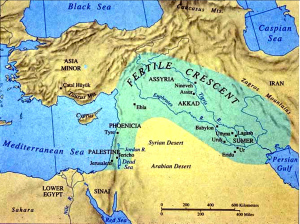
\includegraphics[scale=0.7]{sumermap}
\end{minipage}

\footnotetext{%
	`Between two rivers,' namely the Tigris and Euphrates. As indicated on the map, these rivers formed the backbone of the \emph{fertile crescent,} a region of early civilization, farming, crop and animal domestication.%
}


\boldinline{Sexagesimal (base-60) Positional Enumeration}

Our modern decimal system is \emph{base-10 positional.} This means two things, both of which are easy to see with reference, say, to the number 3835.
\begin{itemize}
	\item The symbol 3 represents both 3000 and 30: the \textbf{meaning of a symbol depends on its position}.
	\item The position of a symbol denotes the \textbf{power of 10} by which it should be multiplied. Thus
	\[
		\textcolor{blue}{3835} =\textcolor{blue}{3}\cdot 10^3 +\textcolor{blue}{8}\cdot 10^2 +\textcolor{blue}{3}\cdot 10^1 +\textcolor{blue}{5}\cdot 10^0
	\]
\end{itemize}
Positional enumeration makes for efficient calculations and easy representation of numbers of vastly different magnitude. Contrast with the difficulty of performing calculations using (non-positional) Egyptian hieroglyphic notation.\smallbreak

One of the key Babylonian contributions to mathematical history is the creation of (arguably) the first positional system of enumeration, dating to at least 2000\BC. Rather than our ten symbols 0--9, Babylonians used only two: roughly $\bone$ for 1 and $\bten$ for 10, likely made by the same stylus. Any number up to 59 could be written with combinations of these symbols, e.g.,\par
\begin{minipage}[t]{0.8\linewidth}\vspace{-10pt}
	\[
		53=
		\begin{array}{c}
			\bten\!\bten\!\bten\\[-5pt]
			\bten\!\bten
		\end{array}
		\hspace{-7pt}
		\bone\!\bone\!\bone
	\]
\end{minipage}
\hfill
\begin{minipage}[t]{0.19\linewidth}\vspace{0pt}
	\flushright
	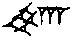
\includegraphics{babylon53}
\end{minipage}
\medbreak
The picture shows a typical cuneiform representation. Larger numbers were represented base-60. For instance, the sexagesimal decomposition of 3835 is
\[
	3835=\textcolor{red}{1}\cdot 60^2+\textcolor{red}{3}\cdot 60^1+\textcolor{red}{55}\cdot 60^0
\]
which the Babylonians would have written
\[
	\vee\quad \vee\!\vee\!\vee\quad 
	\begin{array}{c}
		\bten\!\bten\!\bten\\[-5pt]
		\bten\!\bten
	\end{array}
	\hspace{-8pt}
	\begin{array}{c}
		\bone\!\bone\!\bone\\[-5pt]
		\bone\!\bone
	\end{array}
	\tag{$\ast$}
\]
Rather than using cuneiform, we'll instead write $\textcolor{red}{1},\textcolor{red}{3},\textcolor{red}{55};$

\goodbreak

Just as, for us, `3' might mean 30, 3000 or even $\frac 3{1000}$, for the Babylonians $\vee$ could mean 1, 60, 3600, 216000, or fractions such as $\frac 1{60},\frac 1{3600}$ depending on its position. There was no symbol for zero (as a placeholder) until very late in Babylonian history, nor any \emph{sexagesimal point,} so determining position on ancient tablets can be difficult. For instance, rather than 3835, ($\ast$) might instead have represented
\[
	60+3+\tfrac{55}{60}=63\tfrac{11}{12}\quad\text{or}\quad 60^3+3\cdot 60^2+55\cdot 60=230100
\]
To make things easier to read, we use commas to separate terms and, if necessary, a semicolon to denote the sexagesimal point. Thus
\[
	23,12,0;15=23\cdot 60^2+12\cdot 60+\frac{15}{60}=83520\frac 14
\] 

\boldinline{Why base-60?}

There are many theories, but we cannot be certain. Here are some ideas.
\begin{itemize}
  \item The Babylonians might have combined two systems (base-10 and base-12) inherited from older cultures.
  \item Since 60 has many proper divisors (1, 2, 3, 4, 5, 6, 10, 12, 15, 20, 30), more numbers have exact representation than with decimal arithmetic: for instance $\frac 13=\,;20$, as a terminating sexagesimal, is much simpler than the decimal $0.33333$.
  \item As prolific astronomers and astrologers, the Babylonians might have chosen 60 as a divisor of 360, approximately the number of days in a year. Our modern usage of \emph{degrees-minutes-seconds} for angle, \emph{hours-minutes-seconds} for time, and the standard zodiac are all of Babylonian origin. Indeed Babylonian units of measure often used factors of 60 for magnitude similarly to how modern science uses 1000 (e.g., joules $\rightarrow$ kilojoules $\rightarrow$ megajoules). 
\end{itemize}
This sort of historical question is rarely answerable in a satisfying way. Likely no-one `decided' to use base-60; like most cultural issues, it likely happened slowly and organically, without fanfare.


\boldinline{Basic Sexagesimal Calculations}\phantomsection\label{babmult}

Addition and subtraction would have been as natural to the Babylonians as decimal calculations are to us. For instance, we might write
\[
	\begin{array}{rr@{,\,}r}
		&21&49\\
		+&\underset{\textcolor{red}{1}}{3}&37\\\hline
		&24&26\\
	\end{array} 
	\tag{in decimals $1309+217=1526$}
\]
Note how we \textcolor{red}{carry 60} just like we are used to doing with 10 in decimal arithmetic: $49+37=\textcolor{red}{1},26$.
\smallbreak

Multiplication is significantly harder. To mimic our familiar long-multiplication process would require memorizing up to the 59 times table! For small factors this might have been fine. For larger factors there is evidence of the Babylonians using two representations of a product in terms of squares
\[
	xy=\frac 12\bigl[(x+y)^2-x^2-y^2\bigr]=\frac 14\bigl[(x+y)^2-(x-y)^2\bigr]
\]
Tablets consisting of tables of squares greatly aided the computation of large products. For instance,
\[
	31\times 22 =\frac 14\bigl[53^2-9^2\bigr] 
	=\frac 14\bigl[46,49-1,21\bigr] 
	=\frac 14\bigl[45,28\bigr] 
	=11,7+15=11,22 \tag{$=682$}
\]


\goodbreak


\boldinline{Fractions \& Division}\phantomsection\label{babfraction}

As we've already seen, the Babylonians also represented non-integers using sexagesimals. Tables of reciprocals $\frac 1n$ were used to quickly evaluate division using multiplication!
\[
	m\div n=m\times \frac 1n
\]
For example
\[
	\frac 1{18}=0;3,20 \implies \frac{23}{18}=23(0;3,20) =1;9+0;7,40 =1;16,40
\]
This works nicely provided $n$ has no prime divisors other than 2, 3 or 5, since any such $\frac 1n$ will be an exact terminating sexagesimal.\footnote{%
	Analogous to the fact that $\frac 1n$ has a terminating decimal if and only if $n$ has no prime divisors other than 2 or 5.%
}
Approximations were used for other reciprocals; a scribe would choose a nearby denominator with an exact sexagesimal and state that the answer was approximate
\[
	\frac{11}{29}\approx\frac{11}{30}=11(0;2)=0;22
\]
For more accuracy, one could choose a larger denominator. For instance, if a scribe wanted to divide by 11, they might observe that $11\cdot 13=143\approx 144$, from which\footnote{%
	Being rational, $\frac 1{11}=0.09090909\ldots=0;\textcolor{blue}{5,27,16,21,49,\,}5,27,16,21,49,\ldots$ has a periodic sexagesimal expansion as can be found using a pocket-calculator:
	\[
		\frac{60}{11}=\textcolor{blue}{5}+\frac 5{11},\quad 
		\frac{5\cdot 60}{11}=\textcolor{blue}{27}+\frac 3{11},\quad 
		\frac{3\cdot 60}{11}=\textcolor{blue}{16}+\frac{4}{11},\quad 
		\frac{4\cdot 60}{11}=\textcolor{blue}{21}+\frac{9}{11},\ldots
	\]%
}
\[
	\frac 1{144}=0;0,25\implies \frac 1{11}\approx\frac{13}{144}=0;5,25
\]
Scribes were explicit in acknowledging the approximation by stating, say, ``11 does not divide.'' Remember that a single digit in the second sexagesimal place means only $\frac 1{3600}$, so even the most demanding application doesn't require many terms (the above is 99.3\%{} accurate!).  The denominators in some of these reciprocal tables were enormous, so far greater accuracy was often possible.
\medbreak


Another table listed all the ways an integer $<10$ could be multiplied exactly to get 10.
\[
	\begin{array}{@{}cl@{\qquad\qquad}cl}
		1&10&5&2\\
		2&5&6&1\ 40\\
		3&3\ 20&8&1\ 15\\
		4&2\ 30&9&1\ 6\ 40
\end{array}
\]
We omit the commas for separation and the sexagesimal point as they did not exist. Moreover 7 is missing since $\frac 17$ (and thus $\frac{10}7$) is not an exact sexagesimal. It should be clear from the table that
\[
	\frac{10}6=1;40\quad\text{and}\quad \frac{600}9=1,6;40
\]
In the latter case, note that $600=10\cdot 60$ would be written the same as 10, so this amounts to moving the sexagesimal point in $\frac{10}9=1;6,40$.


\goodbreak


\boldinline{Linear Systems of Equations}

These could be solved by a combination of the method of false position (guess and modify as per the Egyptians) and the consideration of homogeneous equations. For instance, here is a (suitably modernized) Babylonian approach to solving the system
\[
	\begin{cases}
		3x+2y=11\\
		2x+y=7
	\end{cases}
\]
\begin{enumerate}
  \item Choose one equation, say the second, and set $\hat x=\hat y$. Solve this (say using false position) to obtain $\hat x=\hat y=\frac 73=2;20$.
  \item Since $(d,-2d)$ is the general solution to the homogeneous equation $2x+y=0$, all solutions to the second equation have the form $x=\hat x+d$ and $y=\hat y-2d$. Substitute into the first equation:
  \[
  	11=3\left(\frac 73+d\right)+2\left(\frac 73-2d\right)=11+\frac 23-d\implies d=\frac 23
  \]
  \item Finally compute $x=\hat x+d=\frac 73+\frac 23=3$ and $y=\hat y-2d=\frac 73-\frac 43=1$.
\end{enumerate}
Step 2 should should remind you of the `nullspace' method from modern linear algebra: all solutions to the matrix equation $(2\ 1)\stwovec xy=7$ have the form
\[
	\twovec xy=\twovec{x_0}{y_0}+\vn
\]
where $\stwovec{x_0}{y_0}$ is some particular solution (here $x_0=y_0=\frac 73$) and $\vn=\stwovec d{-2d}$ lies in the nullspace of the (row) matrix $(2\ 1)$.


\boldinline{The Yale Tablet (YBC 7289) and Square-root Approximations}\phantomsection\label{ybc7289}

One of the most famous tablets concerns an approximation to $\sqrt 2$. YBC stands for the \emph{Yale Babylonian Collection} which contains over 45,000 objects. YBC 7289 is shown below alongside an enhanced representation of the numerals.
\begin{center}
	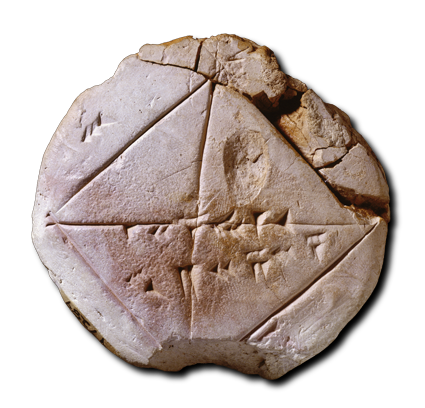
\includegraphics[height=160pt]{YBC7289.png}
	\qquad
	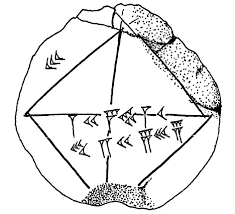
\includegraphics[height=140pt]{ybc.png}
\end{center}

The tablet depicts a square of side 30 and labels the diagonal in two ways:
\begin{itemize}\itemsep0pt
  \item $1;24,51,10$ is an approximation to $\sqrt 2$, an underestimate by roughly 1 part in 2.5 million!
  \item $42;25,35$ is an approximation to the diagonal when the side is 30.
\end{itemize}
The Babylonians more often used the simpler approximation $1;25=1.41666\ldots$ which is still very close. Given the impractical accuracy of YBC 7289, it is reasonable to ask how it was found. No-one knows for certain, but two methods are theorized since both were used to solve other problems. It should be stressed that no Babylonian \emph{proofs} of these approaches are known.

\begin{description}\phantomsection\label{babroot}
	\item[1:\lstsp Square root approximation] $\sqrt{a^2\pm b}\approx a\pm\frac b{2a}$. This is essentially the linear approximation from elementary calculus. If one chooses a rational number $a$ whose square is close to 2, then the error will also be small. For instance:
	\begin{itemize}\itemsep6pt
  	\item $\displaystyle\sqrt 2=\sqrt{1+1}\approx 1+\frac 12=1;30$ \hfill($a=1$)
  	\item $\displaystyle\sqrt 2=\sqrt{\left(\frac 43\right)^2+\frac 29}\approx\frac 43+\frac{2/9}{8/3}=\frac 43+\frac 1{12}=\frac{17}{12}=1;25$ \hfill($a=\frac 43=1.3333\ldots$)
  	\item $\displaystyle\sqrt 2=\sqrt{\left(\frac 75\right)^2+\frac 1{25}}\approx \frac 75+\frac{1/25}{14/5}=\frac{99}{70}=1;24,\textcolor{blue}{51,25,42,}\,51,25,42,\ldots$ \hfill($a=\frac 75=1.4$)
	\end{itemize}
	
	\item[2: Method of the Mean]\phantomsection\label{methodmean} It may be checked (Exercise \ref{exs:methodmean}) that any sequence defined by the recurrence relation $a_{n+1}=\frac 12\left(a_n+\frac 2{a_n}\right)$ converges to $\sqrt 2$. We apply this when $a_1=1$.
	\begin{gather*}
		a_1=1,\quad a_2=\frac 32=1;30,\quad a_3=\frac{17}{12}=1;25\\[6pt]
		a_4=\frac{577}{408}=1+\frac{169}{408}=1;24,51,10,35,17,\ldots\\[6pt]
		a_5=\frac{665857}{470832}=1;24,51,10,7,46\ldots
	\end{gather*}
	It seems incredible that any ancient culture would have bothered to go as far as this to obtain the observed accuracy.\smallbreak

	The same approach can be used to approximate other roots. For example, we can approximate $\sqrt{11}$ via $a_{n+1}=\frac 12(a_n+\frac{11}{a_n})$ and $a_1=3$:
	\[
		a_2=\frac{10}3=3;20,\quad a_3=\frac{199}{60}=3;19,\quad a_4=\frac{79201}{23880}=3;18,59,50,57,17,\ldots
	\]
\end{description}



\boldinline{Quadratic Equations}

The above methods were applied to solve general quadratic equations. A question might be phrased as follows:
\begin{quote}
	I added twice the side to the square; the result is $2,51,40$. What is the side?
\end{quote}
In modern language, we want the solution to $x^2+2x=2\cdot 60^2+51\cdot 60+40=10300$.\smallbreak
Questions such as these were solved using templates, typically as worked examples. The above problem requires the template for solving $x(x+p)=q$ where $p,q>0$. Since the Babylonians did not recognize negative numbers, the other types of quadratic equation ($x^2=px+q$, etc.) had different templates.\goodbreak

To make things a little easier, we apply their approach to the simpler equation $x^2+4x=2$:\smallbreak
Set $y=x+p$ \ ($y=x+4$) and decouple the equation:
\begin{align*}
	&
	\begin{cases}
		xy=q\\
		y-x=p
	\end{cases}
	&&
	\begin{cases}
		xy=2\\
		y-x=4
	\end{cases}
\end{align*}
Use this to solve for $x+y$:
\begin{align*}
	4xy+(y-x)^2&=p^2+4q &4xy+(y-x)^2&=4^2+4\cdot 2\\
	(y+x)^2&=p^2+4q &(y+x)^2&=24\\
	x+y&=\sqrt{p^2+4q} &x+y&=\sqrt{24}\approx\,4;54
\end{align*}
where the square-root was approximated using one of the earlier algorithms, e.g.
\[
	\sqrt{24}=\sqrt{5^2-1}\approx 5-\frac{1}{10}=4;54
\]
Since $x+y$ and $x-y$ are now known, we have a linear system which is easily solved:
\[
	x=\frac{\sqrt{p^2+4q}-p}2 \hspace{50pt} x\approx 0;27
\]
The method of completing the square and the quadratic formula are at least 4000 years old!
\smallbreak
While we've written this abstractly, in practice scribes would be copying from a particular example of the same type. There were no abstract formulæ and everything was done without the benefit modern notation. There was moreover typically no written commentary to explain the method; often all historians have to work with is a single column of numbers!
\smallbreak
Note also that the template only found the positive solution; the Babylonians had no notion of negative numbers. Amazingly, they were able to address certain cubic equations similarly.\smallbreak

\boldinline{Pythagorean Triples}

The Plimpton 322 tablet (also at Yale) lists a large number of Pythagorean triples (albeit with some mistakes). Due to the strange manner of encoding, it took scholars a long time to realize what they had.
	

\begin{minipage}[t]{0.5\linewidth}\vspace{0pt}
	As an example, line 15 describes the Pythagorean triple $53^2=45^2+28^2$:
\begin{itemize}
  \item The first entry $1;23,13,46,40$ is the exact sexagesimal for $\bigl(\frac{53}{45}\bigr)^2$.
  \item The second entry is 28.
  \item The third entry is 53.
  \item The last two entries indicate line number 15.
\end{itemize}
\end{minipage}
\hfill
\begin{minipage}[t]{0.49\linewidth}\vspace{-15pt}
	\flushright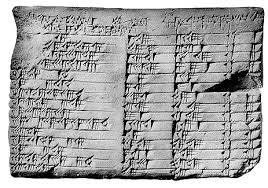
\includegraphics[scale=0.85]{plimpton322.jpg}
\end{minipage}

The first three (interesting) entries are therefore $\bigl((\frac ca)^2,b,c\bigr)$ where $c^2=a^2+b^2$. Since the table is broken on the left side it is possible that a missing column explicitly mentioned $a$.
\smallbreak 

It is not known how the table was completed, though the first column exhibits a descending pattern that provides clues to its construction. One theory is that a scribe found rational solutions to the equation $v^2=1+u^2$ (equivalently $(v+u)(v-u)=1$) by starting with a choice of $v+u$ and using a table of reciprocals to calculate $v-u$.
\smallbreak
To revisit our example, if $v+u=\frac 95=1;48$, then
\[
	v-u=\frac 1{v+u}=\frac 59=0;33,20
\]
We therefore have a linear system of equations in $u,v$ whose solutions are
\[
	v=1;10,40=\frac{53}{45},\quad u=0;37,20=\frac{28}{45}
\]
We investigate this further in Exercise \ref{exs:plimpton}. The Plimpton tablet has been the source of enormous scholarship; look it up!


\boldinline{Geometry}

The Babylonians also considered many geometric problems. They used both $\pi\approx 3$ and $\pi\approx 3\frac 18$ to approximate areas of circles. They had calculations (both correct and erroneous) for the volume of a frustrum (truncated pyramid). They also knew that the altitude of an isosceles triangle bisects its base, and that the angle in semicircle is a right-angle (Thales' Theorem). None of these statements were presented as theorems in a modern sense; we merely have computations and applications that make use of these facts. We simply do not know the depth of Babylonian understanding of such concepts.


\boldsubsubsection{Summary}

\begin{itemize}
  \item Sexagesimal positional enumeration. No zero. Fractions also used sexagesimal representation.
  \item More advanced than Egyptian mathematics but still practical/non-abstract. Perhaps Babylonian mathematics only \emph{appears} more advanced because we have so much more evidence: thousands of tablets versus only a handful of papyri. Like Egypt, we have worked examples without abstraction or statements of general principles.
  \item Some distinction (`does not divide') between approximate and exact results.
  \item Some geometry, but algorithmic/numerical methods predominate.
\end{itemize}



\begin{exercises*}{}{}
	There is no single correct way to do Babylonian calculations. Play with the ideas and use modern  notation to get a feel for things without torturing yourself.
	
	\begin{enumerate}
	  \item %[1-18]
	  Convert the sexagesimal values $0;22,30$, \ $0;8,6$, \ $0;4,10$ and $0;5,33,20$ into ordinary (modern) fractions in lowest terms.
	  
	  
	  \item\begin{enumerate}%[1-20]
	    \item \makebox[220pt][l]{Multiply 25 by $1,4$\hfill(b)}\lstsp Multiply 18 by $1,21$.
	    \item[](\emph{Either compute directly (long multiplication) or use the difference of squares method on page \pageref{babmult}})
	  \end{enumerate}
	  
	  
	  \item\begin{enumerate}%[1-20]
	    \item \makebox[220pt][l]{Use reciprocals to divide 50 by 18.\hfill (b)}\lstsp Repeat for $1,21$ divided by 32.
	  \end{enumerate}
	
	
		\item Use the Babylonian method of false position to solve the linear system $\begin{cases}
		3x+5y=19\\
		2x+3y=12
		\end{cases}$
	  
	  
	  \item%[1-24]
	  \begin{enumerate}
	    \item Convert the approximation $\sqrt 2\approx 1;24,51,10$ to a decimal and verify the accuracy of the approximation on page \pageref{ybc7289}.
	    \item Multiply by 30 to check that the length of the diagonal is as claimed.
	  \end{enumerate}
	  
	  
	  \item Babylonian notation is not required for this question.
	  \begin{enumerate}
	    \item Use the square root approximation (pg.\,\pageref{babroot}) with $a=\frac 83$ to find an approximation to $\sqrt 7$.
	    \item Taking $a_1=3$, apply the method of the mean to find the approximation $a_3$ to $\sqrt 7$.
	  \end{enumerate}
	  
	  
	  \item\label{exs:plimpton}%[1-26]
	  Recall that $v^2=1+u^2$ in the construction of the Plimpton tablet.
	  \begin{enumerate}
	    \item If $v+u=\alpha$, show that $u=\frac 12(\alpha-\alpha^{-1})$ and $v=\frac 12(\alpha+\alpha^{-1})$.
	    \item Suppose $v+u=1;30=\frac 32$. Find $u,v$ and the corresponding Pythagorean triple.
	  	\item Repeat for $v+u=1;52,30=\frac{15}8$.
	  	\item Repeat for $v+u=2;05=\frac{25}{12}$. This is line 9 of the tablet.
	  	%\item Repeat for $v+u=\frac{20}9=2;13,20$.
	  \end{enumerate}
	
	  
	  \item%[1-32] 
	  Solve the following problem from tablet YBC 4652. I found a stone, but did not weigh it; after I subtracted one-seventh, added one-eleventh (of the difference), and then subtracted one-thirteenth (of the previous total), it weighed 1 \emph{mina} ($=60$ \emph{gin}). What was the stone's weight?\par
	  (\emph{The meaning of the problem isn't completely clear: make your best guess!})
	  
	  
	  \item%[1-34]
	  Solve the following problem from tablet YBC 6967. A number exceeds its reciprocal by 7. Find the number and the reciprocal.\par
	  (\emph{In this case, two numbers are reciprocals if their product is 60})
	
	
	  \item For this question it is helpful to think about the corresponding facts for decimals.
	  \begin{enumerate}
	    \item Explain the observation on page \pageref{babfraction} regarding which reciprocals $n$ have a terminating sexagesimal. Can you prove this?
	  	\item Find the periodic sexagesimal representation of $\frac 17$ and use geometric series \emph{prove} that you are correct.
	  \end{enumerate}  
	  
	  
	  \item\label{exs:methodmean}
	  For this question, look up the AM--GM inequality and remind yourself of some basic Analysis.
	  \begin{enumerate}
			\item Suppose $(a_n)$ is a sequence satisfying the recurrence $a_{n+1}=\frac 12(a_n+\frac 2{a_n})$. Prove that $a_n\ge \sqrt 2$ whenever $n\ge 2$.
			\item Prove that $\lim a_n=\sqrt 2$.
		\end{enumerate}
	  
	  
	  
	  \item%[1-22]rephrased
	  \begin{enumerate}
	    \item The Babylonians used an approximation of the form $A\approx\frac 1{12}c^2$ for the area of a circle in terms of its circumference. To what approximation for $\pi$ does this correspond?
	    \item Use a Babylonian method to show that $\sqrt 3\approx\frac 74$.\par
	    \begin{minipage}[t]{0.7\linewidth}\vspace{0pt}
	    	\item A `\textcolor{blue}{bulls-eye}' (pictured) is constructed using congruent circular arcs built from a circumscribed equilateral triangle. If the arc-length is $a$, use Babylonian approximations to prove that the area of the bulls-eye is $\approx\frac{9a^2}{32}$. What, approximately, are its dimensions (width/height)?\par
	    	(\emph{Use as much modern trigonometry as you like!})
	  	\end{minipage}
	  	\hfill
	 		\begin{minipage}[t]{0.25\linewidth}\vspace{-15pt}
	  		\flushright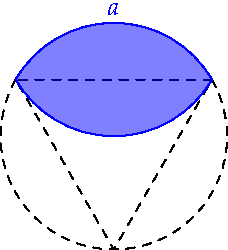
\includegraphics[scale=0.95]{babylon-bullseye}
	  	\end{minipage}
		\end{enumerate}

	  
	\end{enumerate}
\end{exercises*}

% 
% In other situations a two position approximation might be used, for instance
% \[\frac 1{11}=0.09090909\ldots=;5,27,16,21,49,5,27\ldots\]
% which could then be used to divide:
% \[25\div 11=25\cdot(;5,27,16,\ldots)=2;16,21,\ldots\]
% %(working: $25\cdot 16=400=6;40$, $25\cdot 27=675=11;15$, $25\cdot 5=125=2;5$).
% Similarly,
% \[\frac 17=0.142857142857\ldots=;8,34,17,8,34,17,\ldots\]
% yields
% \[10\div 7=10\cdot(;8,34,17,\ldots)=1;25,42,\ldots\]